\documentclass[11pt,a4paper]{report}
\usepackage[textwidth=37em,vmargin=30mm]{geometry}
\usepackage{calc,xunicode,amsmath,amssymb,paralist,enumitem,tabu,booktabs,datetime2,xeCJK,xeCJKfntef,listings}
\usepackage{tocloft,fancyhdr,tcolorbox,xcolor,graphicx,eso-pic,xltxtra,xelatexemoji}

\newcommand{\envyear}[0]{2025}
\newcommand{\envdatestr}[0]{2025-06-15}
\newcommand{\envfinaldir}[0]{webdb/2025/20250615/final}

\usepackage[hidelinks]{hyperref}
\hypersetup{
    colorlinks=false,
    pdfpagemode=FullScreen,
    pdftitle={Web Digest - \envdatestr}
}

\setlength{\cftbeforechapskip}{10pt}
\renewcommand{\cftchapfont}{\rmfamily\bfseries\large\raggedright}
\setlength{\cftbeforesecskip}{2pt}
\renewcommand{\cftsecfont}{\sffamily\small\raggedright}

\setdefaultleftmargin{2em}{2em}{1em}{1em}{1em}{1em}

\usepackage{xeCJK,xeCJKfntef}
\xeCJKsetup{PunctStyle=plain,RubberPunctSkip=false,CJKglue=\strut\hskip 0pt plus 0.1em minus 0.05em,CJKecglue=\strut\hskip 0.22em plus 0.2em}
\XeTeXlinebreaklocale "zh"
\XeTeXlinebreakskip = 0pt


\setmainfont{Brygada 1918}
\setromanfont{Brygada 1918}
\setsansfont{IBM Plex Sans}
\setmonofont{JetBrains Mono NL}
\setCJKmainfont{Noto Serif CJK SC}
\setCJKromanfont{Noto Serif CJK SC}
\setCJKsansfont{Noto Sans CJK SC}
\setCJKmonofont{Noto Sans CJK SC}

\setlength{\parindent}{0pt}
\setlength{\parskip}{8pt}
\linespread{1.15}

\lstset{
	basicstyle=\ttfamily\footnotesize,
	numbersep=5pt,
	backgroundcolor=\color{black!5},
	showspaces=false,
	showstringspaces=false,
	showtabs=false,
	tabsize=2,
	captionpos=b,
	breaklines=true,
	breakatwhitespace=true,
	breakautoindent=true,
	linewidth=\textwidth
}






\newcommand{\coverpic}[2]{
    % argv: itemurl, authorname
    Cover photo by #2~~(\href{#1}{#1})
}
\newcommand{\makeheader}[0]{
    \begin{titlepage}
        % \newgeometry{hmargin=15mm,tmargin=21mm,bmargin=12mm}
        \begin{center}
            
            \rmfamily\scshape
            \fontspec{BaskervilleF}
            \fontspec{Old Standard}
            \fontsize{59pt}{70pt}\selectfont
            WEB\hfill DIGEST
            
            \vfill
            % \vskip 30pt
            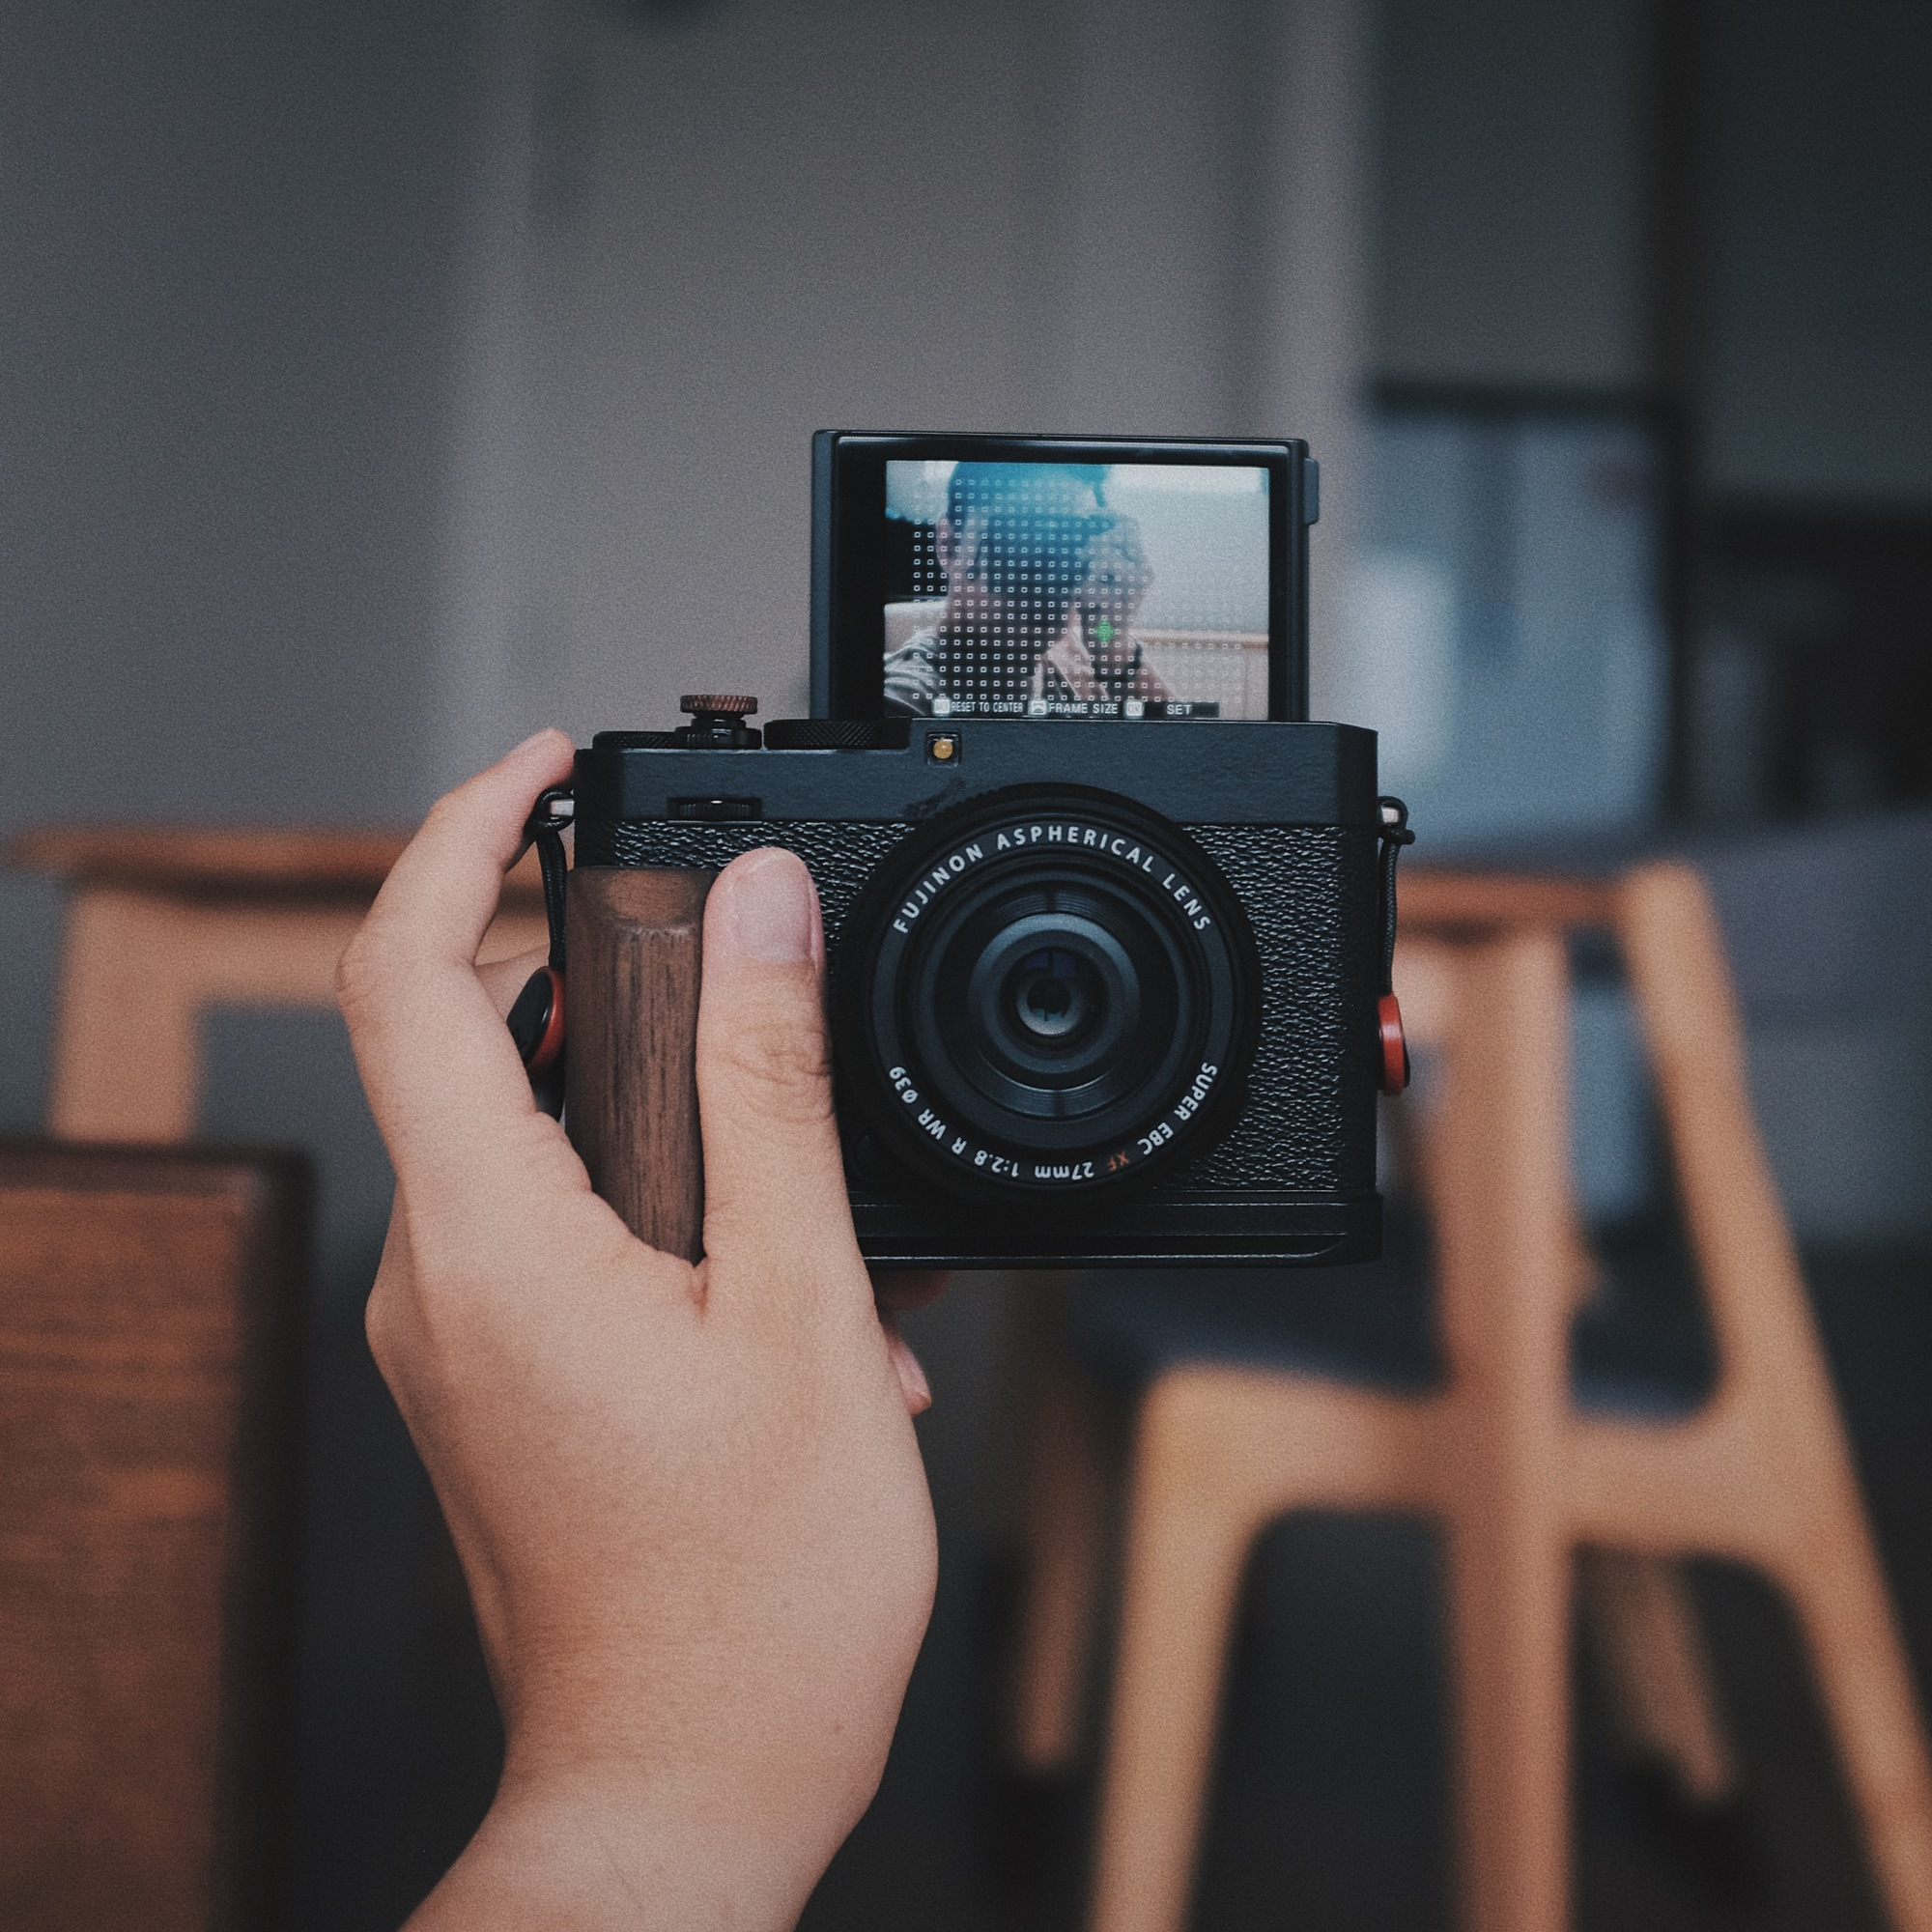
\includegraphics[width=\linewidth]{\envfinaldir/coverpic-prod.jpg}\par
            % \vskip 30pt
            \vfill

            \normalsize\rmfamily\scshape
            \copyright{} The Web Digest Project \hfill\large \envdatestr
        \end{center}
    \end{titlepage}
    % \restoregeometry
}
\newcommand{\simplehref}[1]{%
    \textcolor{blue!80!green}{\href{#1}{#1}}%
}
\renewcommand{\contentsname}{\center\Huge\sffamily\bfseries Contents\par\vskip 20pt}
\newcounter{ipartcounter}
\setcounter{ipartcounter}{0}
\newcommand{\ipart}[1]{
    % \vskip 20pt
    \clearpage
    \stepcounter{ipartcounter}
    \phantomsection
    \addcontentsline{toc}{chapter}{#1}
    % \begin{center}
    %     \Huge
    %     \sffamily\bfseries
    %     #1
    % \end{center}
    % \vskip 20pt plus 7pt
}
\newcounter{ichaptercounter}
\setcounter{ichaptercounter}{0}
\newcommand{\ichapter}[1]{
    % \vskip 20pt
    \clearpage
    \stepcounter{ichaptercounter}
    \phantomsection
    \addcontentsline{toc}{section}{\numberline{\arabic{ichaptercounter}}#1}
    \begin{center}
        \Huge
        \sffamily\bfseries
        #1
    \end{center}
    \vskip 20pt plus 7pt
}
\newcommand{\entrytitlefont}[1]{\subsection*{\raggedright\Large\sffamily\bfseries#1}}
\newcommand{\entryitemGeneric}[2]{
    % argv: title, url
    \parbox{\linewidth}{
        \entrytitlefont{#1}\par\vskip 5pt
        \footnotesize\ttfamily\mdseries
        \simplehref{#2}
    }\vskip 11pt plus 11pt minus 1pt
}
\newcommand{\entryitemGithub}[3]{
    % argv: title, url, desc
    \parbox{\linewidth}{
        \entrytitlefont{#1}\par\vskip 5pt
        \footnotesize\ttfamily\mdseries
        \simplehref{#2}\par\vskip 5pt
        \small\rmfamily\mdseries#3
    }\vskip 11pt plus 11pt minus 1pt
}
\newcommand{\entryitemAp}[3]{
    % argv: title, url, desc
    \parbox{\linewidth}{
        \entrytitlefont{#1}\par\vskip 5pt
        \footnotesize\ttfamily\mdseries
        \simplehref{#2}\par\vskip 5pt
        \small\rmfamily\mdseries#3
    }\vskip 11pt plus 11pt minus 1pt
}
\newcommand{\entryitemHackernews}[3]{
    % argv: title, hnurl, rawurl
    % \parbox{\linewidth}{
    %     \entrytitlefont{#1}\par\vskip 5pt
    %     \footnotesize\ttfamily\mdseries
    %     \simplehref{#3}\par
    %     \textcolor{black!50}{\href{#2}{#2}}
    % }\vskip 11pt plus 11pt minus 1pt
    \begin{minipage}{\linewidth}
            \entrytitlefont{#1}\par\vskip 5pt
            \footnotesize\ttfamily\mdseries
            \simplehref{#3}\par
            \textcolor{black!50}{\href{#2}{#2}}
    \end{minipage}\par\vskip 11pt plus 11pt minus 1pt
}







\begin{document}

\makeheader

\tableofcontents\clearpage




\ipart{Developers}
\ichapter{Hacker News}
\entryitemTwoLinks{Seven replies to the viral Apple reasoning paper and why they fall short}{https://news.ycombinator.com/item?id=44278403}{https://garymarcus.substack.com/p/seven-replies-to-the-viral-apple}

\entryitemTwoLinks{Waymo's market share in San Francisco exceeds Lyft's}{https://news.ycombinator.com/item?id=44277355}{https://underscoresf.com/in-san-francisco-waymo-has-now-bested-lyft-uber-is-next/}

\entryitemTwoLinks{Inside the Apollo "8-Ball" FDAI (Flight Director / Attitude Indicator)}{https://news.ycombinator.com/item?id=44277051}{https://www.righto.com/2025/06/inside-apollo-fdai.html}

\entryitemTwoLinks{I have reimplemented Stable Diffusion 3.5 from scratch in pure PyTorch}{https://news.ycombinator.com/item?id=44276476}{https://github.com/yousef-rafat/miniDiffusion}

\entryitemTwoLinks{Unsupervised Elicitation of Language Models}{https://news.ycombinator.com/item?id=44276041}{https://arxiv.org/abs/2506.10139}

\entryitemTwoLinks{Model Once, Represent Everywhere: UDA (Unified Data Architecture) at Netflix}{https://news.ycombinator.com/item?id=44275575}{https://netflixtechblog.com/uda-unified-data-architecture-6a6aee261d8d}

\entryitemTwoLinks{Last fifty years of integer linear programming: Recent practical advances}{https://news.ycombinator.com/item?id=44274567}{https://inria.hal.science/hal-04776866v1}

\entryitemTwoLinks{Google Cloud Incident Report – 2025-06-13}{https://news.ycombinator.com/item?id=44274563}{https://status.cloud.google.com/incidents/ow5i3PPK96RduMcb1SsW}

\entryitemTwoLinks{\$100 Hamburger}{https://news.ycombinator.com/item?id=44274031}{https://en.wikipedia.org/wiki/\$100\_hamburger}

\entryitemTwoLinks{SIMD-friendly algorithms for substring searching (2018)}{https://news.ycombinator.com/item?id=44274001}{http://0x80.pl/notesen/2016-11-28-simd-strfind.html}

\entryitemTwoLinks{Filedb: Disk-based key-value store inspired by Bitcask}{https://news.ycombinator.com/item?id=44273857}{https://github.com/rajivharlalka/filedb}

\entryitemTwoLinks{The Tech Job Meltdown}{https://news.ycombinator.com/item?id=44273790}{https://www.professoraxelrod.com/p/the-tech-job-meltdown}

\entryitemTwoLinks{Endometriosis is an interesting disease}{https://news.ycombinator.com/item?id=44272933}{https://www.owlposting.com/p/endometriosis-is-an-incredibly-interesting}

\entryitemTwoLinks{Implementing Logic Programming}{https://news.ycombinator.com/item?id=44272467}{https://btmc.substack.com/p/implementing-logic-programming}

\entryitemTwoLinks{Apple's Liquid Glass is prep work for AR interfaces, not just a design refresh}{https://news.ycombinator.com/item?id=44271630}{https://omc345.substack.com/p/from-skeuomorphic-to-liquid-glass}

\entryitemTwoLinks{Self-Adapting Language Models}{https://news.ycombinator.com/item?id=44271284}{https://arxiv.org/abs/2506.10943}

\entryitemTwoLinks{I convinced HP's board to buy Palm and watched them kill it}{https://news.ycombinator.com/item?id=44270709}{https://philmckinney.substack.com/p/i-convinced-hps-board-to-buy-palm}

\entryitemTwoLinks{When random people give money to random other people (2017)}{https://news.ycombinator.com/item?id=44270144}{https://quomodocumque.wordpress.com/2017/06/27/when-random-people-give-money-to-random-other-people/}

\entryitemTwoLinks{Peano arithmetic is enough, because Peano arithmetic  encodes computation}{https://news.ycombinator.com/item?id=44269822}{https://math.stackexchange.com/a/5075056/6708}

\entryitemTwoLinks{The Hat, the Spectre and SAT Solvers (2024)}{https://news.ycombinator.com/item?id=44269289}{https://www.nhatcher.com/post/on-hats-and-sats/}\ichapter{Dribbble}
\entryitemGeneric{\hskip 0pt{}Aquasan}{https://dribbble.com/shots/26100535-Aquasan}

\entryitemGeneric{\hskip 0pt{}Eagle}{https://dribbble.com/shots/26099428-Eagle}

\entryitemGeneric{\hskip 0pt{}Mnp Technologies - Logo Design}{https://dribbble.com/shots/26092034-Mnp-Technologies-Logo-Design}

\entryitemGeneric{\hskip 0pt{}Singular Logo Concept (Unused)}{https://dribbble.com/shots/26091755-Singular-Logo-Concept-Unused}

\entryitemGeneric{\hskip 0pt{}Cre8tera // Website}{https://dribbble.com/shots/26091009-Cre8tera-Website}

\entryitemGeneric{\hskip 0pt{}Cool Pool Logo Design - Letter C Monogram}{https://dribbble.com/shots/26091401-Cool-Pool-Logo-Design-Letter-C-Monogram}

\entryitemGeneric{\hskip 0pt{}Gorilla + Bar Chart Logo}{https://dribbble.com/shots/26092670-Gorilla-Bar-Chart-Logo}

\entryitemGeneric{\hskip 0pt{}zeero logo design}{https://dribbble.com/shots/26087342-zeero-logo-design}

\entryitemGeneric{\hskip 0pt{}Create email inbox composition}{https://dribbble.com/shots/26083118-Create-email-inbox-composition}

\entryitemGeneric{\hskip 0pt{}Shori Brand}{https://dribbble.com/shots/26088139-Shori-Brand}

\entryitemGeneric{\hskip 0pt{}Roaring Bear}{https://dribbble.com/shots/26087788-Roaring-Bear}

\entryitemGeneric{\hskip 0pt{}Eagle}{https://dribbble.com/shots/26085536-Eagle}

\entryitemGeneric{\hskip 0pt{}Hand-drawn illustration pack}{https://dribbble.com/shots/26084735-Hand-drawn-illustration-pack}

\entryitemGeneric{\hskip 0pt{}Dog Mascot Various Poses}{https://dribbble.com/shots/26087977-Dog-Mascot-Various-Poses}

\entryitemGeneric{\hskip 0pt{}Branding Concept for Europe}{https://dribbble.com/shots/26087652-Branding-Concept-for-Europe}

\entryitemGeneric{\hskip 0pt{}B2B Dashboard \& Web App UI UX Design for Carbon Solutions}{https://dribbble.com/shots/26076624-B2B-Dashboard-Web-App-UI-UX-Design-for-Carbon-Solutions}

\entryitemGeneric{\hskip 0pt{}Patriot Logo Design (Unused for Sale)}{https://dribbble.com/shots/26081047-Patriot-Logo-Design-Unused-for-Sale}

\entryitemGeneric{\hskip 0pt{}Heliopoint}{https://dribbble.com/shots/26081987-Heliopoint}

\entryitemGeneric{\hskip 0pt{}Apple}{https://dribbble.com/shots/26084067-Apple}

\entryitemGeneric{\hskip 0pt{}Illustration}{https://dribbble.com/shots/26083223-Illustration}

\entryitemGeneric{\hskip 0pt{}Europe Logo Animation}{https://dribbble.com/shots/26082596-Europe-Logo-Animation}

\entryitemGeneric{\hskip 0pt{}Arc Logo}{https://dribbble.com/shots/26083648-Arc-Logo}

\entryitemGeneric{\hskip 0pt{}Heyo Turns 2!}{https://dribbble.com/shots/26078572-Heyo-Turns-2}

\entryitemGeneric{\hskip 0pt{}Fox Brand Mascot}{https://dribbble.com/shots/26077954-Fox-Brand-Mascot}


\ipart{Developers~~~~(zh-Hans)}
\ichapter{Solidot}
\entryitemGeneric{\hskip 0pt{}人类首次拍摄到太阳南极}{https://www.solidot.org/story?sid=81557}

\entryitemGeneric{\hskip 0pt{}因 AI 科技巨头的间接碳排放自 2020 年以来增长了 50\%}{https://www.solidot.org/story?sid=81556}

\entryitemGeneric{\hskip 0pt{}当 Google 打了个喷嚏,全世界都感冒了}{https://www.solidot.org/story?sid=81555}

\entryitemGeneric{\hskip 0pt{}代糖赤藓糖醇被发现会损害脑血管细胞功能}{https://www.solidot.org/story?sid=81554}

\entryitemGeneric{\hskip 0pt{}丹麦一政府部门准备淘汰 Windows 和 Microsoft 365}{https://www.solidot.org/story?sid=81552}

\entryitemGeneric{\hskip 0pt{}研究认为霸王龙的大型化始于亚洲}{https://www.solidot.org/story?sid=81551}

\entryitemGeneric{\hskip 0pt{}两名欧洲记者的手机感染了以色列间谍软件 Paragon}{https://www.solidot.org/story?sid=81550}

\entryitemGeneric{\hskip 0pt{}Scale AI 亚历山大·王的创业法则:人类计算资源可像计算机一样编排,吴恩达一观点毁掉红杉投资,YC创始人一句话带来商业灵感}{https://www.solidot.org/story?sid=81549}

\entryitemGeneric{\hskip 0pt{}Anker 召回逾百万台有起火风险的移动电源}{https://www.solidot.org/story?sid=81545}

\entryitemGeneric{\hskip 0pt{}马斯克威胁起诉广告商取得部分成效}{https://www.solidot.org/story?sid=81544}

\entryitemGeneric{\hskip 0pt{}四天工作制能提高生产力}{https://www.solidot.org/story?sid=81543}

\entryitemGeneric{\hskip 0pt{}谷歌CEO皮查伊两小时访谈:AI是人类所见过最深远的技术,意义将超越火与电,因为它可以自我迭代}{https://www.solidot.org/story?sid=81542}

\entryitemGeneric{\hskip 0pt{}印度航空发生致命空难,至少 200 人死亡}{https://www.solidot.org/story?sid=81541}

\entryitemGeneric{\hskip 0pt{}迪士尼和 NBC 起诉 Midjourney 侵犯版权}{https://www.solidot.org/story?sid=81540}

\entryitemGeneric{\hskip 0pt{}韦伯观测到下沙雨的气态巨行星}{https://www.solidot.org/story?sid=81539}

\entryitemGeneric{\hskip 0pt{}MS Office 的版本控制从 Source Depot 迁移到 Git}{https://www.solidot.org/story?sid=81538}

\entryitemGeneric{\hskip 0pt{}1997年,乔布斯在WWDC闭幕环节做了唯一一场即兴问答:我们要做``更好的产品'',而非``不同的产品'',十年后,iPhone发布}{https://www.solidot.org/story?sid=81537}

\entryitemGeneric{\hskip 0pt{}印度宇航员将搭乘 Axiom Space 的飞船前往国际空间站}{https://www.solidot.org/story?sid=81536}

\entryitemGeneric{\hskip 0pt{}太阳活动与 Starlink 卫星大量坠落相关}{https://www.solidot.org/story?sid=81535}

\entryitemGeneric{\hskip 0pt{}新闻网站来自 Google 的流量大幅下降}{https://www.solidot.org/story?sid=81534}\ichapter{V2EX}
\entryitemGeneric{\hskip 0pt{}[问与答] zen browser 垂直滚动条不贴边怎么破?}{https://www.v2ex.com/t/1138635}

\entryitemGeneric{\hskip 0pt{}[分享创造] 分享一下我前段时间写 的 llms.txt 生成器}{https://www.v2ex.com/t/1138634}

\entryitemGeneric{\hskip 0pt{}[Apple] 有没有开 fitness+ 美区合租车的,想上个年付车}{https://www.v2ex.com/t/1138633}

\entryitemGeneric{\hskip 0pt{}[问与答] 有 ai 辅助后,学习曲线这东西越来越模糊了。}{https://www.v2ex.com/t/1138632}

\entryitemGeneric{\hskip 0pt{}[分享创造] NewSink 部署在 cloudflare 上的短链接/重定向(允许多接入域名)}{https://www.v2ex.com/t/1138631}

\entryitemGeneric{\hskip 0pt{}[OpenAI] 大家现在使用 ChatGPT 是不是速度很慢?}{https://www.v2ex.com/t/1138630}

\entryitemGeneric{\hskip 0pt{}[问与答] 求推荐张 esim 卡应急用,少量流量+外站注册}{https://www.v2ex.com/t/1138629}

\entryitemGeneric{\hskip 0pt{}[程序员] 公司用的 mac ,目前家里是 win. 突然想到是否家里也换个 mac 代码放到 cloud 里面}{https://www.v2ex.com/t/1138628}

\entryitemGeneric{\hskip 0pt{}[Local LLM] 多卡部署 QWQ Q8 是否可行}{https://www.v2ex.com/t/1138625}

\entryitemGeneric{\hskip 0pt{}[宽带症候群] 上海移动用京东自营路由器无法联网}{https://www.v2ex.com/t/1138624}

\entryitemGeneric{\hskip 0pt{}[问与答] 想找一款可以用 gd、od 或国内网盘同步的订阅到期提醒 app}{https://www.v2ex.com/t/1138623}

\entryitemGeneric{\hskip 0pt{}[程序员] 码云 Gitee 终于下线仓库 star 接口了}{https://www.v2ex.com/t/1138622}

\entryitemGeneric{\hskip 0pt{}[Python] Resolver 模式,一种比 GraphQL 适用于 BFF 的新选择}{https://www.v2ex.com/t/1138620}

\entryitemGeneric{\hskip 0pt{}[硬件] 360 门铃 tf 卡满后,无法格式化是卡坏了吗?看 bbs 有很人也遇到类似问题,是 360 门铃设计缺陷? https://bbs.360.cn/thread-15094602-1-1.html}{https://www.v2ex.com/t/1138619}

\entryitemGeneric{\hskip 0pt{}[骑行] 求助,关于新手第一辆公路车的选择}{https://www.v2ex.com/t/1138618}

\entryitemGeneric{\hskip 0pt{}[Swift] Swift DocC 构建的博客}{https://www.v2ex.com/t/1138615}

\entryitemGeneric{\hskip 0pt{}[小米] 有办法解决小米平板有线投屏电视黑边问题吗?}{https://www.v2ex.com/t/1138612}

\entryitemGeneric{\hskip 0pt{}[云修电脑] 分享一下最近遇到的内存超频问题}{https://www.v2ex.com/t/1138611}

\entryitemGeneric{\hskip 0pt{}[宽带症候群] 最近几天发现上海电信 拨号上网 有分配 ipv6 地址了}{https://www.v2ex.com/t/1138610}

\entryitemGeneric{\hskip 0pt{}[宽带症候群] 抖音导致 Pppoe 被强制 T 下线}{https://www.v2ex.com/t/1138608}

\entryitemGeneric{\hskip 0pt{}[路由器] 求教。MT3000 要如何设置透明代理?}{https://www.v2ex.com/t/1138606}

\entryitemGeneric{\hskip 0pt{}[程序员] wsl2 上搞安卓 rom 开发,舒服吗?}{https://www.v2ex.com/t/1138604}

\entryitemGeneric{\hskip 0pt{}[HomeKit] homekit 摄像头视频流只支持 1080p?}{https://www.v2ex.com/t/1138602}

\entryitemGeneric{\hskip 0pt{}[Android] 请教一下, Pixel9 内置 Pixel studio 在根目录中的位置?}{https://www.v2ex.com/t/1138600}

\entryitemGeneric{\hskip 0pt{}[互联网] 爬取小红书评论是否合法}{https://www.v2ex.com/t/1138599}

\entryitemGeneric{\hskip 0pt{}[问与答] 非认证的微信公众号、小程序、公众平台,是否有办法实现 H5 页面支持微信登录?}{https://www.v2ex.com/t/1138598}

\entryitemGeneric{\hskip 0pt{}[开源软件] 有哪些开源项目是比较值得捐赠的?}{https://www.v2ex.com/t/1138596}

\entryitemGeneric{\hskip 0pt{}[Kubernetes] [远程] 急招中高级运维(k8s 方向)薪资 14k-18k}{https://www.v2ex.com/t/1138595}

\entryitemGeneric{\hskip 0pt{}[问与答] 最近公司组织爱心献血,有些个人疑问}{https://www.v2ex.com/t/1138594}

\entryitemGeneric{\hskip 0pt{}[OpenAI] 被 gpt 气到了!}{https://www.v2ex.com/t/1138593}

\entryitemGeneric{\hskip 0pt{}[问与答] 我用 iphone15 连 win11 的热点,过段时间就连不上网,什么原因}{https://www.v2ex.com/t/1138591}

\entryitemGeneric{\hskip 0pt{}[Linux] 如何使用 fdisk 创建正确的 swap 分区?}{https://www.v2ex.com/t/1138590}

\entryitemGeneric{\hskip 0pt{}[问与答] [有偿] 在腾讯云上使用 Docker Compose 部署的前后端项目,连接数据库失败}{https://www.v2ex.com/t/1138589}

\entryitemGeneric{\hskip 0pt{}[微信] PC 端还在用 3.x 版本,最近已经直接收到 4.x 版本的升级提醒了}{https://www.v2ex.com/t/1138588}

\entryitemGeneric{\hskip 0pt{}[问与答] IOS 端怎么把网页转成 App?}{https://www.v2ex.com/t/1138587}

\entryitemGeneric{\hskip 0pt{}[问与答] TrafficMonitor 代替品有什么推荐的?}{https://www.v2ex.com/t/1138586}

\entryitemGeneric{\hskip 0pt{}[分享发现] Liquid Glass CSS 生成器上线,可自定义 iOS 26 风格 UI,支持导出 HTML/CSS}{https://www.v2ex.com/t/1138585}

\entryitemGeneric{\hskip 0pt{}[问与答] Bing 把我站点索引都清空了}{https://www.v2ex.com/t/1138583}

\entryitemGeneric{\hskip 0pt{}[生活] 4 年多没登录了,看到了之前的帖子感慨万千}{https://www.v2ex.com/t/1138580}

\entryitemGeneric{\hskip 0pt{}[奇思妙想] Closet Craft (虚拟衣橱 + AI 穿搭)}{https://www.v2ex.com/t/1138578}

\entryitemGeneric{\hskip 0pt{}[创业组队] 初创组队,招募小游戏主程/美工/设计合伙人 - 北京}{https://www.v2ex.com/t/1138577}

\entryitemGeneric{\hskip 0pt{}[iPhone] 微信未登录下怎么备份聊天记录}{https://www.v2ex.com/t/1138576}

\entryitemGeneric{\hskip 0pt{}[Apple] Apple 家庭组 music 共享问题}{https://www.v2ex.com/t/1138575}

\entryitemGeneric{\hskip 0pt{}[Apple] itunes 怎么老是要把我的专辑分裂成两张}{https://www.v2ex.com/t/1138573}

\entryitemGeneric{\hskip 0pt{}[程序员] ArkFlow+ Python : 轻松实现实时 AI}{https://www.v2ex.com/t/1138569}

\entryitemGeneric{\hskip 0pt{}[Android] 如何正确配置代理使 FCM 保持长期连接、或直接走直连?}{https://www.v2ex.com/t/1138567}

\entryitemGeneric{\hskip 0pt{}[投资] ChatGPT 选股还是有点用的}{https://www.v2ex.com/t/1138564}

\entryitemGeneric{\hskip 0pt{}[Google] gemini 苦旅 - 伊斯坦布尔}{https://www.v2ex.com/t/1138562}

\entryitemGeneric{\hskip 0pt{}[程序员] 请问有没有什么办法能批量把 docx 格式转成 doc 格式}{https://www.v2ex.com/t/1138561}

\entryitemGeneric{\hskip 0pt{}[分享创造] 从 360 安全到独立开发:我的第一个海外产品 Face Fat Analysis}{https://www.v2ex.com/t/1138560}


\ipart{Generic News}
\ichapter{Reuters}
\entryitemWithDescription{\hskip 0pt{}Russia and Ukraine exchange prisoners of war}{https://www.reuters.com/world/europe/russia-ukraine-exchange-prisoners-war-moscow-received-no-war-dead-russia-says-2025-06-14/}{Moscow did not receive any of its war dead from Kyiv, Russian state media...}

\entryitemWithDescription{\hskip 0pt{}King Charles honours air crash victims at military parade}{https://www.reuters.com/business/aerospace-defense/king-charles-honours-air-crash-victims-military-parade-2025-06-14/}{Britain\textquotesingle s King Charles and other senior royals wore black armbands at the "Trooping the Colour" military parade on Saturday as a mark of respect for the victims of the Air India plane...}

\entryitemWithDescription{\hskip 0pt{}Lebanon will keep its airspace open, minister says}{https://www.reuters.com/world/middle-east/lebanon-will-keep-its-airspace-open-minister-says-2025-06-14/}{Lebanon will aim to keep its airspace open, a minister said on Saturday, hours after officials said the airspace would be shut down in the evening amid Iran-Israel...}

\entryitemWithDescription{\hskip 0pt{}Seoul's LGBT community gathers for annual festival after liberal president elected}{https://www.reuters.com/world/asia-pacific/seouls-lgbt-community-gathers-annual-festival-after-liberal-president-elected-2025-06-14/}{The annual Seoul Queer Culture Festival was held in the South Korean capital on Saturday after the country ushered in a new liberal president, though it faced concurrent protests against the LGBT community\textquotesingle s pride...}

\entryitemWithDescription{\hskip 0pt{}Ukraine receives 1,200 bodies of dead Ukrainian soldiers, Kyiv says}{https://www.reuters.com/business/aerospace-defense/ukraine-receives-1200-bodies-dead-ukrainian-soldiers-kyiv-says-2025-06-14/}{Ukraine has received 1,200 bodies of its soldiers killed in the war with Russia, Ukrainian officials responsible for exchanging prisoners of war said on...}

\entryitemWithDescription{\hskip 0pt{}Israeli fire kills 23 people in Gaza, many at aid site, medics say}{https://www.reuters.com/world/middle-east/israeli-fire-kills-23-people-gaza-many-aid-site-medics-say-2025-06-14/}{Israeli fire and airstrikes killed at least 23 Palestinians across the Gaza Strip, most of them near an aid distribution site operated by the U.S.-backed Gaza Humanitarian Foundation, local health authorities...}

\entryitemWithDescription{\hskip 0pt{}Zelenskiy says Ukraine halts Russian troops' advance in Sumy region}{https://www.reuters.com/business/aerospace-defense/zelenskiy-says-ukraine-halts-russian-troops-advance-sumy-region-2025-06-14/}{Ukraine\textquotesingle s president said that troops maintained their defensive lines along more than 1,000 kilometers of the...}

\entryitemWithDescription{\hskip 0pt{}Canada's Sikhs voice outrage over Modi G7 invitation}{https://www.reuters.com/world/americas/canadas-sikhs-voice-outrage-over-modi-g7-invitation-2025-06-14/}{Members of Canada\textquotesingle s Sikh community who were warned by police that their lives were at risk and allege the Indian government is responsible for the threat are incensed by Ottawa\textquotesingle s invitation to Prime...}

\entryitemWithDescription{\hskip 0pt{}Protests, Middle East - and bad weather - may rain on Trump's military parade}{https://www.reuters.com/business/aerospace-defense/protests-middle-east-bad-weather-may-rain-trumps-military-parade-2025-06-14/}{Anti-Trump groups are planning to hold nearly 2,000 demonstrations across the U...}

\entryitemWithDescription{\hskip 0pt{}Iraq reopens Syria crossing for trade and passenger traffic}{https://www.reuters.com/world/middle-east/iraq-reopens-syria-crossing-trade-passenger-traffic-2025-06-14/}{Iraq has officially reopened the Qaim border crossing with Syria for trade and passenger traffic, a spokesman for the Iraqi border authority said on Saturday, marking a key step in efforts to normalise relations and revive economic ties...}

\entryitemWithDescription{\hskip 0pt{}Austria plans tougher gun laws after mass shooting at school}{https://www.reuters.com/business/media-telecom/austria-plans-tougher-gun-laws-after-mass-shooting-school-2025-06-14/}{The Austrian government plans to tighten national gun laws after enduring its worst school shooting, Chancellor Christian Stocker said in an interview broadcast on...}

\entryitemWithDescription{\hskip 0pt{}Pope Leo appeals for 'reason' amid Israel-Iran airstrikes, calls for dialogue}{https://www.reuters.com/world/europe/pope-leo-appeals-reason-amid-israel-iran-airstrikes-calls-dialogue-2025-06-14/}{Pope Leo appealed on Saturday for authorities in Iran and Israel to act with "reason" after airstrikes between the two countries killed dozens and sent civilians into shelters, and called on the nations to pursue...}

\entryitemWithDescription{\hskip 0pt{}Iran vows to continue strikes against Israel, US bases, military officials say}{https://www.reuters.com/world/middle-east/iran-vows-continue-strikes-against-israel-us-bases-military-officials-say-2025-06-14/}{Iran\textquotesingle s strikes against Israel will continue, with targets set to expand to include U.S. bases in the region in the coming days, Iran\textquotesingle s Fars news agency reported on Saturday, citing senior Iranian military...}






\clearpage
\leavevmode\vfill
\footnotesize

Copyright \copyright{} 2023-2025 Neruthes and other contributors.

This document is published with CC BY-NC-ND 4.0 license.

The entries listed in this newsletter may be copyrighted by their respective creators.

This newsletter is generated by the Web Digest project.

The newsletters are also delivered via Telegram channel \CJKunderline{\href{https://t.me/webdigestchannel}{https://t.me/webdigestchannel}}.\\
RSS feed is available at \CJKunderline{\href{https://webdigest.pages.dev/rss.xml}{https://webdigest.pages.dev/rss.xml}}.

This newsletter is available in PDF at
\CJKunderline{\href{https://webdigest.pages.dev/}{https://webdigest.pages.dev/}}.

The source code being used to generate this newsletter is available at\\
\CJKunderline{\href{https://github.com/neruthes/webdigest}{https://github.com/neruthes/webdigest}}.

This newsletter is also available in
\CJKunderline{\href{http://webdigest.pages.dev/readhtml/\envyear/WebDigest-20250615.html}{HTML}} and
\CJKunderline{\href{https://github.com/neruthes/webdigest/blob/master/markdown/\envyear/WebDigest-20250615.md}{Markdown}}.


\coverpic{https://unsplash.com/photos/a-beautiful-dome-of-a-magnificent-church-Wya6thlv4ys}{Francis Nie}


\end{document}
